\chapter{Empirical Evaluation}
\label{chapter4}
Within this chapter, we evaluate our various implementations in a collection of gridworld-like domains. The goal of the evaluation is to see how effectively our agents can explore and learn against baseline methods. 

% Furthermore, we perform some ablation studies to evaluate how important certain elements of our framework are to success. We finish by evaluating how well our agents are able to generalise to differing tasks within a domain.

\section{Baselines}
In order to truly evaluate our framework implementations, we needed some baselines to compare against. Firstly, we chose $\epsilon$-greedy, with simulated annealing, due to its ubiquity. Secondly, we chose "PRL", a model-based exploration method that always acts greedily with respect to current model during exploration, which is updated through observations; this is essentially our framework minus the Meta Actions, and is explained quite well by Algorithm \ref{alg:framework_pc}. 
This was chosen as we wanted to evaluate the usefulness of Meta Actions.

% We decided not to compare against SOTA algorithms discussed in the literature review, as due to their complexities they would prove difficult to implement. 
% Furthermore, it didn't seem like a fair comparison, as we made various simplifications when implementing our framework.

\section{Domains}
The domains that we chose to evaluate within were all gridworld-based. This decision was made due to the ease of modelling such domains, especially in a tabular manner. Furthermore, this enabled us to easily understand how the agents explore. Thus, the actions available to the agents are common between tasks (unless specified otherwise); up, down, left and right. Where Meta Actions are not learned, reasonable ones are specified that enable the agent to hypothesise changes between rewards and transitions among adjacent states. The Manhattan Distance \cite{krause1973taxicab} is used as a heuristic in agents that utilise A*.
\\Gridworld is a deterministic domain, shown in Figure \ref{fig:grid_domain}. The agent starts in the middle of the room at the bottom of the grid. There are three doors to leave the room, in the left, right and top of the room. All of the doors are open, if they were closed then the agent would not know how to open them. The goal of the agent is to navigate to the other side of the top door. In our experiments, the model that the agents were seeded with indicated that the door leading to the goal was closed. The agent receives a reward of -1 at every time step.
\\Cliff-Walking \cite{Sutton1998} is a deterministic domain, shown in Figures \ref{fig:cliff_walking} and \ref{fig:cliff_walking_openai}. The agent starts in the bottom left corner of the grid and needs to navigate to the goal state at the bottom right of the grid. However, there is a cliff along the bottom of the grid, which the agent needs to avoid. In our experiments, the model that the agents were seeded with indicated that the cliff was bigger than it actually is; it was along the bottom two rows of the grid. The agent receives a reward of -1 at every time step, unless it steps into the cliff which induces a reward of -100 and returns the agent to the start state (without terminating the episode).
\\Windy-Gridworld \cite{Sutton1998} is a deterministic domain, shown in Figure \ref{fig:windy_gridworld} The agent starts in the left middle of the grid, and must navigate towards a goal state on the right-hand side of the grid. However, the is an upward wind within some columns which varies in strength. The wind shifts the next state upwards by the strength of the wind. In our experiments, the model that the agents were seeded with did not capture the wind. The agent receives a reward of -1 at every time step.
\\Stochastic Gridworld is the same as Gridworld, except there is some stochasticity introduced; the top door has a probability of 0.4 of being closed, within each episode. In our experiments, the model that the agents were seeded with indicated that the door leading to the goal was closed, with probability 1. The reward formulation and the actions available to the agent remain the same along with the seeded model.
\\Frozen Lake \cite{1606.01540} is a stochastic domain, shown in Figure \ref{fig:frozen_lake}. The agent must navigate from the start state in the top-left corner to the goal state in the bottom-right corner. However, the frozen lake is slippery, meaning that the agent moves in the intended direction with probability $\frac{1}{3}$ and in either of the perpendicular directions with probability $\frac{1}{3}$ each. Furthermore, there are holes where the ice has been broken or melted and entering these holes terminate the episode. The model that the agents were seeded with did not capture the slipperiness of the frozen lake, and also suggests that there is only a single path to the goal state. Rewards are sparse; reaching the goal state returns a reward of +1, whilst at all other time steps the agent receives no reward.
\\Stochastic Windy-Gridworld is the same as Windy-Gridworld, except there is stochasticity introduced;  the wind (if there is any) is stochastic. The reward formulation and the actions available to the agent remain the same along with the seeded model.

% \section{Evaluation Metrics}
% \begin{itemize}
%     \item Learning Curve
%     \item Sample efficiency? 
% \end{itemize}
\section{Results \& Analysis}
Within this section, we present results of evaluating our implementations against the aforementioned domains. All results were generated by aggregating over 20 runs, where each run produced a sliding window view, with a window size 5. Thus, each point plotted represents the average over the previous 5 episodes averaged over the 20 runs. An outlier to this was the Frozen Lake domain, where a window size of $1$ was used. These decisions were made to reduce variance in the results due to randomness, and overall produce a more robust set of results. We also plot the 95\% confidence intervals. Throughout all experiments, a discount factor of 1.0 was used, due to the episodic nature of the domains. Moreover, a learning rate of $0.6$ was used; this was tuned by-hand and turned out to produce the best results for all agents. For the model-based agents, a maximum of $10$ planning steps was allotted.
\\Figures \ref{fig:deterministic_results} and \ref{fig:stochastic_results} present the learning curves for each agent in each of the deterministic and stochastic domains, respectively. Tables \ref{table:deterministic_results} and \ref{tab:example_table} provide summaries of these results, including the minimum, mean, maximum and final rewards, as well as the standard deviation.
\\\textbf{Gridworld} \quad In the Gridworld domain, the agent that performed best on average was RL A* Meta (RLAM), closely followed by RL VI Meta (RLVIM). The poorest performing was the RL agent, which accumulated a fair amount of negative reward in the initial episodes. During the Planning phase, RLAM and RLVIM were each able to discover the optimal policy, however the formed did it much quicker. The PRL and RL VI Meta Learn (RLVIML) agents followed the exact same path throughout the planning phase, and didn't diverge from it; this was because the PRL agent didn't experience any discprencies between its model and the domain and thus didn't replan, whilst the RLVIML agent did not actually learn any Meta Actions to utilise. Each of the model-based agents suffered considerable performance decreases whilst switching to the learnt $Q$ values. All of the agents were able to discover the optimal policy within the 100 episode limit.
\\\textbf{Windy Gridworld} \quad In the Windy Gridworld domain, the RLVIM agent outperformed the others on average, although it was closely followed by the RLAM and PRL agents. The RL agent again struggled during its initial exploration, accruing large negative rewards. While the RLAM and PRL agents were able to discover the optimal policy during exploration, the RLVIM agent was not, although it seems to have explored more thoroughly since it suffered less during the switch to the model-free learning. The RLVIML agent was not successful at all; the Meta Actions that it learned somehow led to it becoming stuck in local optima during planning and unable to complete even a single episode. Interestingly, the RLAM and PRL agents were able to achieve a maximum reward of -15.0, which is in-fact optimal, however the agent performing the best in the end was the RL agent; this may be due to insufficient exploration.
\\\textbf{Cliff-Walking} \quad In the Cliff-Walking domain, the RLVIM agent was once again the best performing on average, by some distance. It seems to have performed the best during the exploratory phase; its attempts at reasoning about the environment led to it discovering the true-cliff, enabling it to avoid it later on, and thus it didn't see too much of a drop in performance when switching to model-free learning. The RL agent again struggled with its initial exploration, with its inital performance being around a factor of a 100 worst than the other agents; this is likely due to dithering, causing the agent to step into the cliff. The RLAM and PRL agents did not perform much exploration, leading to large dips in performance once again. Furthermore, the RLVIML agent wasn't successful in learning any Meta Actions, so it performed very similarly to PRL. By the final episode all agents, but the RL agent, were able to discover the optimal policy.
\\\textbf{Stochastic Gridworld}  \quad In the Stochastic Gridworld, the PRL agent performed the best on average; although it did not perform much exploration in comparison to the other agents. Compellingly, the RLVIM agent did not suffer from the performance dip witnessed in previous domains; perhaps this is because it indeed achieved sufficient exploration. The RL agent once again accumulated considerable negative reward during its initial exploration. The RLVIML and RL A* Meta short term memory (RLAM STM) agents were completely unsuccessful. Interestingly, the successful agents learned a policy that didn't use the door, although it was open more often than not.
\\\textbf{Stochastic Windy Gridworld} \quad In the Stochastic Windy Gridworld domain, the pure RL agent achieved the best performance, followed closely by the PRL agent. In this domain, the RLVIM agent accumulated more negative reward than the RL agent during their respective initial explorations. The RLVIML and RL A* Meta short term memory (RLAMSTM) agents were completely unsuccessful, again. However, the other agents learned relatively stable policies, and were able to deal with the stochasticity well.
\\\textbf{Frozen Lake} \quad In the Frozen Lake domain, the PRL agent achieved the best performance, although all of the agents performed generally poor; achieving a maximum of 3.75\% success. In this domain, the RLVIML agent outperformed RLVIM by a small margin, this is interesting and indicates that useful Meta Actions were learned. The RLAMSTM agent failed to complete a single episode.
\\In conclusion, the model-based agents generally outperformed the pure RL agent; and the Meta agent variations tended to outperform the plain PRL agent. For the most part, all of the agents were able to learn good policies with a limited number of episodes. Learning reasonable Meta Actions didn't prove to be very successful, however using embedded Meta Actions was quite successful. The RLAMSTM agent failed in every domain; this may be due to the cost function that we formulated for the agent, and it might've been more successful if we determinised the model and used our deterministic version of A* (see Section \ref{sec:rlam}). All of the model-based agents typically displayed considerable decreases in performance when switching to model-free learning - this is caused by some states having never been visited during exploration. 

% Some states are certainly not-optimal and therefore its okay not to visit them. However, it would have been much better if we found a way to avoid this performance dip.
% \\Figure \ref{fig:stochastic_results} presents the learning curves for each agent in each of the stochastic domains. We note however that the cumulative reward is plotted for the Frozen Lake domain, due to its sparse reward signal. Table \ref{tab:example_table} provides a summary of these results, including the min, mean, max, final rewards and the standard deviation in the rewards. Within the 

% \textbf{Stochastic Gridworld} domain, the best performing agent on average was the PRL agent. However, the PRL agent once again did not perform much exploration, whereas the other agents did. The RL agent again struggled during exploration, accumulating very negative rewards. Interestingly, all agents learned a policy that doesn't use the door, even though it is open more often than not. I

% n the Stochastic Windy Gridworld domain, the best performing agent on average was the RL agent, interestingly. However, while all agents struggled with the high stochasticity they were able to learn relatively stable policies. 

% Within the \textbf{Frozen Lake} domain, the PRL agent once again performed the best. Interestingly, the RLVIML agent outperformed its counterpart that does not learn Meta Actions. The RL agent was the worst performing. In general, the agents didn't perform too well in this small, but difficult domain, achieving a maximum of 3.75\% success.


% \\For the deterministic domains, we present the learning curves for each agent in each domain in Figure \ref{fig:deterministic_results}. We also present a summary of the results, including the min, max, mean and final reward, as well as the standard deviation of the rewards, in Table \ref{table:deterministic_results}.
% \\For the stochastic domains, we also present the learning curves and a summary of the results in Figure \ref{fig:stochastic_results} and Table \ref{tab:example_table} respectively.

\begin{figure}[H]
    \centering
    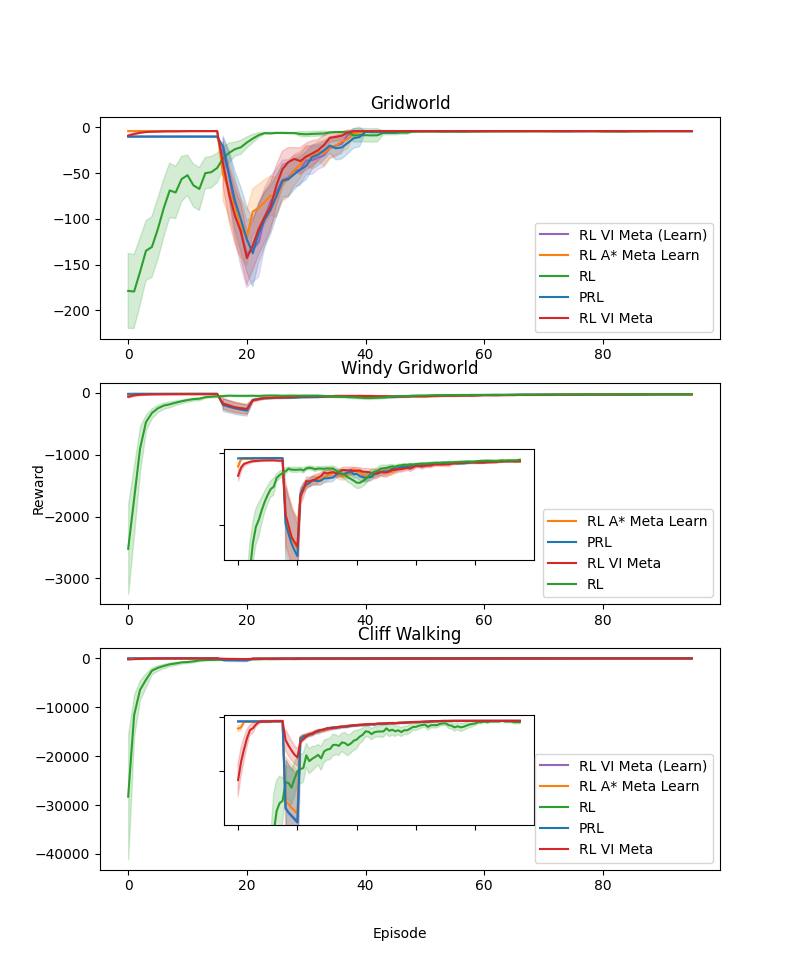
\includegraphics[max size={\textwidth}{\textheight}]{report/assets/deterministic_results.png}
    \caption{Deterministic Results}
    \label{fig:deterministic_results}
\end{figure}


\begin{figure}[H]
    \centering
    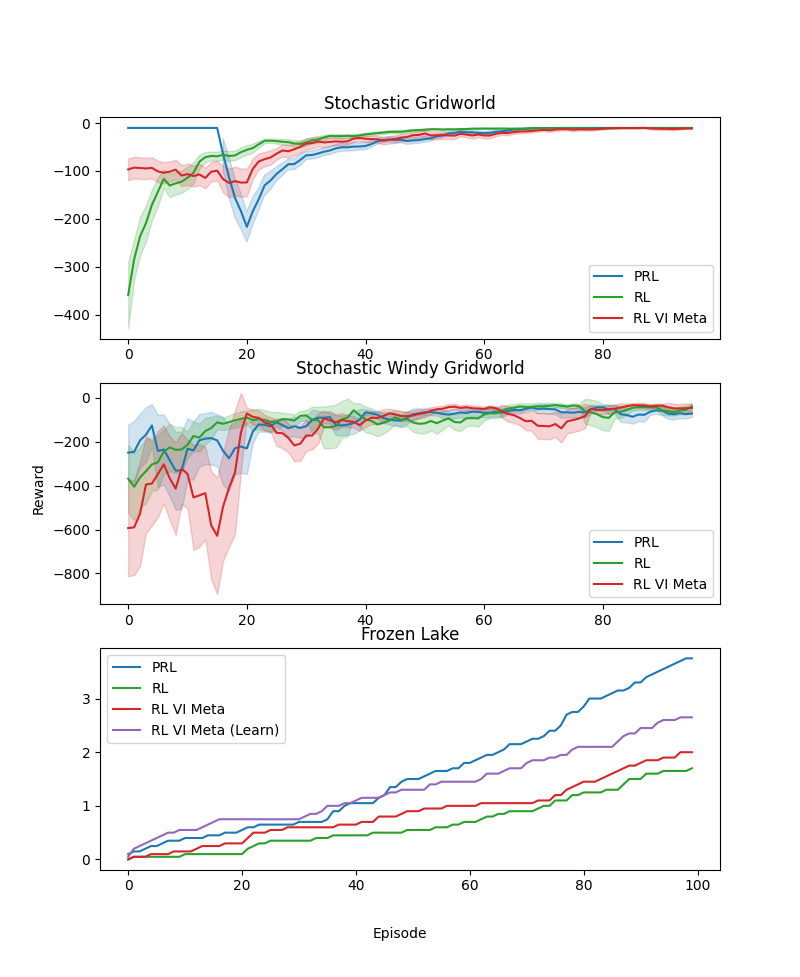
\includegraphics[max size={\textwidth}{\textheight}]{report/assets/stochastic_results.png}
    \caption{Stochastic Results}
    \label{fig:stochastic_results}
\end{figure}

\begin{table}[h]
\centering
\begin{tabular}{|c|c|c|c|}
\hline
\textbf{Agent} & \textbf{Gridworld} & \textbf{Windy Gridworld} & \textbf{Cliff-Walking}\\ \hline
\textbf{RLVIM} & 
\begin{tabular}{|c|c|}
\hline
Min & -209.72 \\ \hline
Max & -10.0 \\ \hline
Mean & -16.24 \\ \hline
Std. Dev & 29.743 \\ \hline
Final & -4.0 \\ \hline
\end{tabular}& 
\begin{tabular}{|c|c|}
\hline
Min & -259.3 \\ \hline
Max & -20.9 \\ \hline
Mean & -50.152 \\ \hline
Std. Dev & 44.944\\ \hline
Final & -23.62 \\ \hline
\hline
\end{tabular}&
\begin{tabular}{|c|c|}
\hline
Min & -231.64 \\ \hline
Max & -13.0 \\ \hline
Mean & -34.258 \\ \hline
Std. Dev & 37.456 \\ \hline
Final & -13.0 \\ \hline
\end{tabular} \\ \hline
\textbf{RLVIM (Learn)} & 
\begin{tabular}{|c|c|}
\hline
Min & -138.42 \\ \hline
Max & -4.0 \\ \hline
Mean & -18.111 \\ \hline
Std. Dev & 30.005 \\ \hline
Final & -4.0 \\ \hline
\end{tabular}& 
\begin{tabular}{|c|c|}
\hline
Min & DNF \\ \hline
Max & DNF \\ \hline
Mean & DNF \\ \hline
Std. Dev & DNF \\ \hline
Final & DNF \\ \hline
\end{tabular}& 
\begin{tabular}{|c|c|}
\hline
Min & -383.74 \\ \hline
Max & -13.0 \\ \hline
Mean & -40.66 \\ \hline
Std. Dev & 76.498 \\ \hline
Final & -13.0 \\ \hline
\end{tabular} \\ \hline
\textbf{RLAM} & 
\begin{tabular}{|c|c|}
\hline
Min & -120.58 \\ \hline
Max & -4.0 \\ \hline
Mean & -16.111 \\ \hline
Std. Dev & 26.631 \\ \hline
Final & -4.0 \\ \hline
\end{tabular}& 
\begin{tabular}{|c|c|}
\hline
Min & -267.0, \\ \hline
Max & -15.0 \\ \hline
Mean & -50.375 \\ \hline
Std. Dev & 47.226 \\ \hline
Final & -23.8 \\ \hline
\end{tabular}& 
\begin{tabular}{|c|c|}
\hline
Min & -357.08 \\ \hline
Max & -13.0 \\ \hline
Mean & -39.78 \\ \hline
Std. Dev & 70.261 \\ \hline
Final & -13.0 \\ \hline
\end{tabular} \\ \hline
\textbf{PRL} & 
\begin{tabular}{|c|c|}
\hline
Min & -137.58 \\ \hline
Max & -4.0 \\ \hline
Mean & -18.017 \\ \hline
Std. Dev & 28.838 \\ \hline
Final & -4.0 \\ \hline
\end{tabular}& 
\begin{tabular}{|c|c|}
\hline
Min & -286.64 \\ \hline
Max & -15.0 \\ \hline
Mean & -51.018 \\ \hline
Std. Dev & 51.16 \\ \hline
Final & -23.16 \\ \hline
\end{tabular}& 
\begin{tabular}{|c|c|}
\hline
Min & -388.7 \\ \hline
Max & -13.0 \\ \hline
Mean & -40.635 \\ \hline
Std. Dev & 77.127 \\ \hline
Final & -13.0 \\ \hline
\end{tabular} \\ \hline
\textbf{RL} & 
\begin{tabular}{|c|c|}
\hline
Min & -179.46 \\ \hline
Max & -4.0 \\ \hline
Mean & -21.012 \\ \hline
Std. Dev & 38.013 \\ \hline
Final & -4.06 \\ \hline
\end{tabular}& 
\begin{tabular}{|c|c|}
\hline
Min & -2521.54 \\ \hline
Max & -19.16 \\ \hline
Mean & -109.037 \\ \hline
Std. Dev &  317.461 \\ \hline
Final & -19.16 \\ \hline
\end{tabular}& 
\begin{tabular}{|c|c|}
\hline
Min & -28279.32 \\ \hline
Max & -13.2 \\ \hline
Mean & -709.696 \\ \hline
Std. Dev & 3170.597 \\ \hline
Final & -17.54 \\ \hline
\end{tabular} \\ \hline
\end{tabular}
\caption{Reward Summary for Deterministic Domains}
\label{table:deterministic_results}
\end{table}


\begin{table}[h]
\centering
\begin{tabular}{|c|c|c|c|}
\hline
\textbf{Agent} & \textbf{Stoch. Gridworld} & \textbf{Stoch. Windy Gridworld} & \textbf{Frozen Lake}\\ \hline
\textbf{RLVIM} & 
\begin{tabular}{|c|c|}
\hline
Min & -125.0 \\ \hline
Max & -9.92 \\ \hline
Mean & -44.666 \\ \hline
Std. Dev & 36.761 \\ \hline
Final & -10.92 \\ \hline
\end{tabular}& 
\begin{tabular}{|c|c|}
\hline
Min & -628.3 \\ \hline
Max & -32.9 \\ \hline
Mean & -155.688 \\ \hline
Std. Dev & 153.302\\ \hline
Final & -45.5 \\ \hline
\end{tabular}&
\begin{tabular}{|c|c|}
\hline
Success Rate & 2.0\%\\\hline
\end{tabular} \\ \hline
\textbf{RLVIM (Learn)} & 
\begin{tabular}{|c|c|}
\hline
Min & DNF\\ \hline
Max & DNF \\ \hline
Mean & DNF \\ \hline
Std. Dev & DNF \\ \hline
Final & DNF \\ \hline
\end{tabular}& 
\begin{tabular}{|c|c|}
Min & DNF \\ \hline
Max & DNF \\ \hline
Mean & DNF \\ \hline
Std. Dev & DNF \\ \hline
Final & DNF \\ \hline
\end{tabular}& 
\begin{tabular}{|c|c|}
\hline
Success Rate & 2.65\%\\\hline
\end{tabular} \\ \hline
\textbf{RLAM (STM)} & 
\begin{tabular}{|c|c|}
\hline
Min & DNF \\ \hline
Max & DNF \\ \hline
Mean & DNF \\ \hline
Std. Dev & DNF \\ \hline
Final & DNF \\ \hline
\end{tabular}& 
\begin{tabular}{|c|c|}
\hline
Min & DNF \\ \hline
Max & DNF \\ \hline
Mean & DNF \\ \hline
Std. Dev & DNF \\ \hline
Final & DNF \\ \hline
\end{tabular}& 
\begin{tabular}{|c|c|}
\hline
Success Rate & DNF\\\hline
\end{tabular} \\ \hline
\textbf{PRL} & 
\begin{tabular}{|c|c|}
\hline
Min & -216.72 \\ \hline
Max & -10.0 \\ \hline
Mean & -36.766 \\ \hline
Std. Dev & 43.71 \\ \hline
Final & -10.02 \\ \hline
\end{tabular}& 
\begin{tabular}{|c|c|}
\hline
Min & -331.2 \\ \hline
Max & -43.1 \\ \hline
Mean & -112.641 \\ \hline
Std. Dev & 70.109 \\ \hline
Final & -71.1 \\ \hline
\end{tabular}& 
\begin{tabular}{|c|c|}
\hline
Success Rate & 3.75\%\\\hline
\end{tabular} \\ \hline
\textbf{RL} & 
\begin{tabular}{|c|c|}
\hline
Min & -359.3 \\ \hline
Max & -10.22 \\ \hline
Mean & -42.7 \\ \hline
Std. Dev & 59.999 \\ \hline
Final & -10.22\\ \hline
\end{tabular}& 
\begin{tabular}{|c|c|}
\hline
Min & -405.1 \\ \hline
Max & -32.4 \\ \hline
Mean & -107.711 \\ \hline
Std. Dev &  76.601 \\ \hline
Final & -38.3 \\ \hline
\end{tabular}& 
\begin{tabular}{|c|c|}
\hline
Success Rate & 1.7\%\\\hline
\end{tabular} \\ \hline
\end{tabular}
\caption{Reward Summary for Stochastic Domains}
\label{tab:example_table}
\end{table}


% \begin{table}[h]
% \centering
% \begin{tabular}{|c|c|c|c|}
% \hline
% \textbf{Agent} & \textbf{Gridworld} & \textbf{Cliff-Walking} & \textbf{Windy Gridworld}\\ \hline
% \textbf{RLVIM} &  \hline
% \textbf{RLVIM (Learn)} & \\ \hline
% \textbf{RLAM} & \\ \hline
% \textbf{RL VI} &  \\ \hline
% \textbf{RL} &  \\ \hline
% \end{tabular}
% \caption{Reward Summary for Gridworld}
% \label{tab:example_table}
% \end{table}

% \section{Analysis}

% \section{Ablation Studies}
% \subsection{Learning from Scratch}
% \subsection{Reasonability}
% \section{Generalisation Study}

% \section{Learning from Scratch: An Ablation Study}

% \section{}
